%% ============================================================
%%  LLM-Powered Multi-Agent MLIR to QIR Translator
%%  Beamer Presentation  --  compile with: pdflatex (x2)
%% ============================================================
\documentclass[aspectratio=169,10pt]{beamer}

%% ── Theme ───────────────────────────────────────────────────
\usetheme{Madrid}
\usecolortheme{seahorse}
\setbeamertemplate{navigation symbols}{}
\setbeamertemplate{footline}[frame number]
\setbeamerfont{frametitle}{size=\normalsize,series=\bfseries}

%% ── Packages ────────────────────────────────────────────────
\usepackage[utf8]{inputenc}
\usepackage[T1]{fontenc}
\usepackage{lmodern}
\usepackage{microtype}
\usepackage{listings}
\usepackage{xcolor}
\usepackage{tikz}
\usepackage{pgfplots}
\pgfplotsset{compat=1.18}
\usetikzlibrary{arrows.meta,shapes.geometric,positioning,fit,
                decorations.pathreplacing,calc,backgrounds}
\usepackage{booktabs}
\usepackage{tabularx}
\usepackage{multirow}
\usepackage{amsmath,amssymb}
\usepackage{fontawesome5}
\usepackage{graphicx}
\usepackage{array}
\usepackage{colortbl}

%% ── Custom Colours ──────────────────────────────────────────
\definecolor{mlirblue}{RGB}{0,122,204}
\definecolor{qirgreen}{RGB}{0,160,100}
\definecolor{ssaorange}{RGB}{210,110,0}
\definecolor{condred}{RGB}{190,40,40}
\definecolor{agentpurple}{RGB}{120,50,170}
\definecolor{ragcyan}{RGB}{0,140,170}
\definecolor{codebg}{RGB}{38,42,50}
\definecolor{codegreen}{RGB}{80,200,120}
\definecolor{codeyellow}{RGB}{220,190,70}
\definecolor{codeblue}{RGB}{100,160,220}
\definecolor{codepurple}{RGB}{180,100,220}
\definecolor{codered}{RGB}{220,90,90}

%% ── Listings styles ─────────────────────────────────────────
\lstdefinestyle{mlirstyle}{
  backgroundcolor=\color{codebg},
  basicstyle=\ttfamily\fontsize{6.2}{7.8}\selectfont\color{white},
  keywordstyle=\color{codeblue}\bfseries,
  commentstyle=\color{codegreen}\itshape,
  stringstyle=\color{codeyellow},
  breaklines=true,
  showstringspaces=false,
  frame=single,
  rulecolor=\color{mlirblue},
  framesep=3pt,
  xleftmargin=4pt,
  xrightmargin=2pt,
}
\lstdefinestyle{qirstyle}{
  backgroundcolor=\color{codebg},
  basicstyle=\ttfamily\fontsize{6.2}{7.8}\selectfont\color{white},
  commentstyle=\color{gray}\itshape,
  breaklines=true,
  showstringspaces=false,
  frame=single,
  rulecolor=\color{qirgreen},
  framesep=3pt,
  xleftmargin=4pt,
  xrightmargin=2pt,
}
\lstdefinestyle{pystyle}{
  backgroundcolor=\color{codebg},
  basicstyle=\ttfamily\fontsize{6.2}{7.8}\selectfont\color{white},
  keywordstyle=\color{codepurple}\bfseries,
  commentstyle=\color{codegreen}\itshape,
  stringstyle=\color{codeyellow},
  breaklines=true,
  showstringspaces=false,
  frame=single,
  rulecolor=\color{agentpurple},
  framesep=3pt,
  xleftmargin=4pt,
  xrightmargin=2pt,
}

%% ── Macros ──────────────────────────────────────────────────
\newcommand{\hl}[1]{\textcolor{mlirblue}{\textbf{#1}}}
\newcommand{\hlg}[1]{\textcolor{qirgreen}{\textbf{#1}}}
\newcommand{\hlo}[1]{\textcolor{ssaorange}{\textbf{#1}}}
\newcommand{\hlr}[1]{\textcolor{condred}{\textbf{#1}}}
\newcommand{\hlp}[1]{\textcolor{agentpurple}{\textbf{#1}}}
\newcommand{\hlc}[1]{\textcolor{ragcyan}{\textbf{#1}}}

% Coloured pill badge (no tikz to avoid beamer issues)
\newcommand{\badge}[2]{%
  \colorbox{#1}{\color{white}\tiny\bfseries~#2~}}

%% ── Metadata ─────────────────────────────────────────────────
\title[MLIR $\to$ QIR Translator]{%
  LLM-Powered Multi-Agent MLIR to QIR\\
  Quantum Circuit Translator}
\subtitle{Architecture, Implementation \& Translation Semantics}
\author{Agentic ML/QC Research}
\date{2026}
\institute{PennyLane Catalyst \(\cdot\) CUDA Quantum \(\cdot\) QIR Alliance}

%% ============================================================
\begin{document}
%% ============================================================

\begin{frame}[plain]
  \titlepage
  \begin{tikzpicture}[remember picture,overlay]
    \node[anchor=south east,inner sep=8pt] at (current page.south east){%
      \scriptsize\color{gray}
      33 modules \(\cdot\) 3\,700+ lines \(\cdot\) 7 phases \(\cdot\) 2 dialects};
  \end{tikzpicture}
\end{frame}

\begin{frame}{Table of Contents}
  \tableofcontents
\end{frame}

%% ============================================================
\section{Motivation \& Problem Statement}
%% ============================================================

\begin{frame}{The Quantum IR Landscape}
  \begin{columns}[T]
    \column{0.48\textwidth}
      \textbf{Multiple frameworks produce different IRs}
      \vspace{4pt}
      \begin{block}{Source IRs (MLIR-based)}
        \begin{itemize}
          \item \hl{PennyLane Catalyst:} \texttt{quantum.*} dialect
          \item \hl{CUDA Quantum (Quake):} \texttt{quake.*} dialect
        \end{itemize}
      \end{block}
      \begin{block}{Target IR}
        \begin{itemize}
          \item \hlg{QIR Alliance:} LLVM IR-based
        \end{itemize}
      \end{block}
    \column{0.48\textwidth}
      \textbf{Translation Challenges}
      \begin{alertblock}{Non-trivial semantics}
        \begin{enumerate}\small
          \item \hlo{SSA variable chains} -- qubit indices buried in
                multi-result operations
          \item \hlo{Parametric gates} -- angles as SSA constants,
                not literal values
          \item \hlo{Conditional branching} -- \texttt{scf.if} linked
                to measurements through 5 IR operations
          \item \hlo{Operation ordering} -- gates and measurements
                must be interleaved, not grouped
        \end{enumerate}
      \end{alertblock}
  \end{columns}
\end{frame}

\begin{frame}{Why Naive Regex Fails: The SSA Problem}
  \begin{columns}[T]
    \column{0.50\textwidth}
      \textbf{GHZ-5 CNOT chain in Catalyst MLIR}
      \vspace{4pt}
      \begin{block}{Naive approach (wrong)}
        Extract trailing digit from variable name:\\
        \texttt{\%out\_qubits\_\textbf{1}\#0} $\Rightarrow$ qubit 1\\[4pt]
        \hlr{Result:} CNOT(0,1), CNOT(1,2), CNOT(1,3)\\
        \hlr{Wrong:} control qubit keeps changing
      \end{block}
      \begin{exampleblock}{SSA-aware approach (correct)}
        Trace \texttt{\%out\_qubits\_1\#0} back:\\
        CNOT output\#0 $\leftarrow$ CNOT input\#0\\
        $\leftarrow$ \texttt{\%out\_qubits\_0\#0}\\
        $\leftarrow$ CNOT input\#0\\
        $\leftarrow$ \texttt{\%out\_qubits}\\
        $\leftarrow$ \texttt{extract[0]} $=$ qubit \textbf{0}\\[2pt]
        \hlg{Result:} CNOT(0,1), CNOT(0,2), CNOT(0,3)
      \end{exampleblock}
    \column{0.46\textwidth}
      \begin{center}
      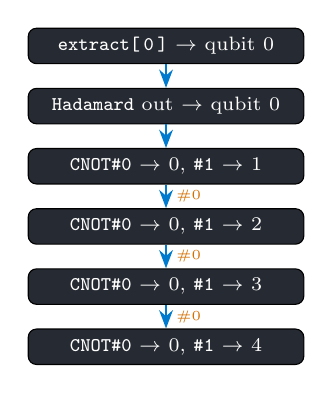
\begin{tikzpicture}[
        box/.style={draw,rounded corners=3pt,minimum width=3.5cm,
                    minimum height=0.45cm,font=\scriptsize,
                    text centered,inner sep=2pt,fill=codebg,
                    text=white},
        arr/.style={-Stealth,thick,mlirblue},
        scale=0.9,
      ]
        \node[box](e0){\texttt{extract[\,0\,]} $\to$ qubit 0};
        \node[box,below=0.3cm of e0](h){\texttt{Hadamard} out $\to$ qubit 0};
        \node[box,below=0.3cm of h](c1){%
          \texttt{CNOT\#0} $\to$ 0, \texttt{\#1} $\to$ 1};
        \node[box,below=0.3cm of c1](c2){%
          \texttt{CNOT\#0} $\to$ 0, \texttt{\#1} $\to$ 2};
        \node[box,below=0.3cm of c2](c3){%
          \texttt{CNOT\#0} $\to$ 0, \texttt{\#1} $\to$ 3};
        \node[box,below=0.3cm of c3](c4){%
          \texttt{CNOT\#0} $\to$ 0, \texttt{\#1} $\to$ 4};
        \draw[arr](e0)--(h);
        \draw[arr](h)--(c1);
        \draw[arr](c1)--(c2)node[midway,right,
          font=\tiny,text=ssaorange]{\#0};
        \draw[arr](c2)--(c3)node[midway,right,
          font=\tiny,text=ssaorange]{\#0};
        \draw[arr](c3)--(c4)node[midway,right,
          font=\tiny,text=ssaorange]{\#0};
      \end{tikzpicture}
      \end{center}
      \vspace{2pt}
      \centering\small Each \texttt{\#0} carries qubit 0 forward
  \end{columns}
\end{frame}

%% ============================================================
\section{System Architecture}
%% ============================================================

\begin{frame}{Seven-Phase Architecture Overview}
  \begin{center}
  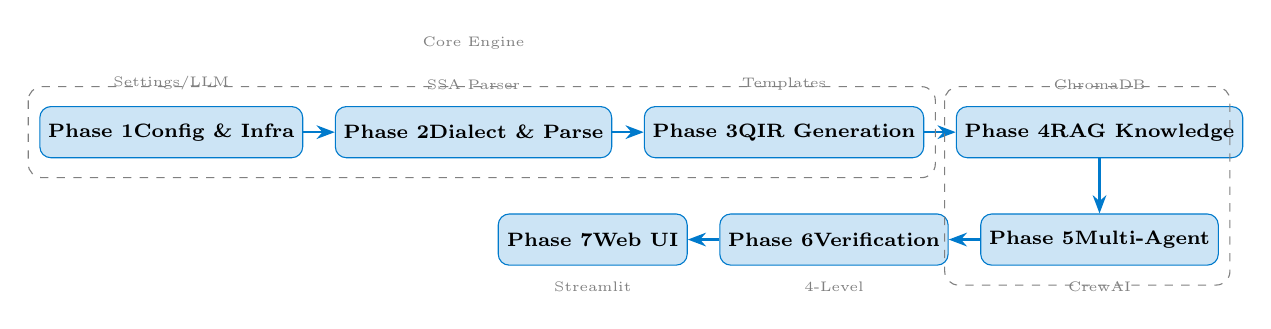
\begin{tikzpicture}[
    box/.style={draw,rounded corners=4pt,minimum width=2.4cm,
                minimum height=0.65cm,font=\scriptsize\bfseries,
                text centered,inner sep=3pt,fill=mlirblue!20,
                draw=mlirblue},
    arr/.style={-Stealth,thick,mlirblue},
  ]
    \node[box,align=center](p1){Phase 1\newline Config \& Infra};
    \node[box,align=center,right=0.4cm of p1](p2){Phase 2\newline Dialect \& Parse};
    \node[box,align=center,right=0.4cm of p2](p3){Phase 3\newline QIR Generation};
    \node[box,align=center,right=0.4cm of p3](p4){Phase 4\newline RAG Knowledge};
    \node[box,align=center,below=0.7cm of p4](p5){Phase 5\newline Multi-Agent};
    \node[box,align=center,left=0.4cm of p5](p6){Phase 6\newline Verification};
    \node[box,align=center,left=0.4cm of p6](p7){Phase 7\newline Web UI};
    \draw[arr](p1)--(p2); \draw[arr](p2)--(p3);
    \draw[arr](p3)--(p4); \draw[arr](p4)--(p5);
    \draw[arr](p5)--(p6); \draw[arr](p6)--(p7);
    \node[above=0.08cm of p1,font=\tiny\color{gray}]{Settings/LLM};
    \node[above=0.08cm of p2,font=\tiny\color{gray}]{SSA Parser};
    \node[above=0.08cm of p3,font=\tiny\color{gray}]{Templates};
    \node[above=0.08cm of p4,font=\tiny\color{gray}]{ChromaDB};
    \node[below=0.08cm of p5,font=\tiny\color{gray}]{CrewAI};
    \node[below=0.08cm of p6,font=\tiny\color{gray}]{4-Level};
    \node[below=0.08cm of p7,font=\tiny\color{gray}]{Streamlit};
    \draw[dashed,gray,rounded corners=5pt]
      ([xshift=-4pt,yshift=7pt]p1.north west) rectangle
      ([xshift=4pt,yshift=-7pt]p3.south east);
    \node[above=0.6cm of p2,font=\tiny\color{gray}]{Core Engine};
    \draw[dashed,gray,rounded corners=5pt]
      ([xshift=-4pt,yshift=7pt]p4.north west) rectangle
      ([xshift=4pt,yshift=-7pt]p5.south east);
  \end{tikzpicture}
  \end{center}
  \vspace{8pt}
  \begin{columns}[T]
    \column{0.32\textwidth}
      \leavevmode\textbf{Core (Phases 1--3)}

      \smallskip Deterministic, rule-based translation engine
    \column{0.32\textwidth}
      \leavevmode\textbf{AI Layer (Phases 4--5)}

      \smallskip RAG-enhanced LLM agents with iterative refinement
    \column{0.32\textwidth}
      \leavevmode\textbf{QA Layer (Phases 6--7)}

      \smallskip 4-level verification and Streamlit web interface
  \end{columns}
\end{frame}

\begin{frame}{End-to-End Data Flow}
  \begin{center}
  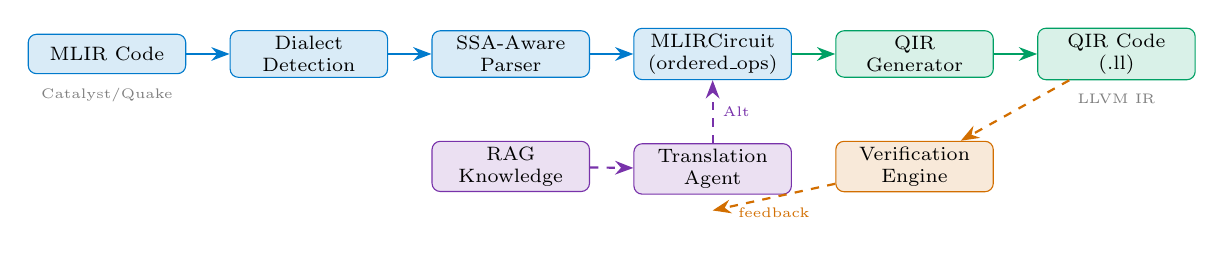
\begin{tikzpicture}[
    node distance=0.4cm and 0.55cm,
    box/.style={draw,rounded corners=3pt,minimum width=2.0cm,
                minimum height=0.5cm,font=\scriptsize,
                text centered,inner sep=2pt},
    arr/.style={-Stealth,thick},
    ds/.style={box,fill=mlirblue!15,draw=mlirblue},
    ps/.style={box,fill=qirgreen!15,draw=qirgreen},
    as/.style={box,fill=agentpurple!15,draw=agentpurple},
    vs/.style={box,fill=ssaorange!15,draw=ssaorange},
  ]
    \node[ds](mlir){MLIR Code};
    \node[ds,right=of mlir,align=center](detect){Dialect\\Detection};
    \node[ds,right=of detect,align=center](parse){SSA-Aware\\Parser};
    \node[ds,right=of parse,align=center](circuit){MLIRCircuit\\(ordered\_ops)};
    \node[ps,right=of circuit,align=center](gen){QIR\\Generator};
    \node[ps,right=of gen,align=center](qir){QIR Code\\(.ll)};
    \node[as,below=0.8cm of parse,align=center](rag){RAG\\Knowledge};
    \node[as,below=0.8cm of circuit,align=center](agent){Translation\\Agent};
    \node[vs,below=0.8cm of gen,align=center](verify){Verification\\Engine};
    \draw[arr,mlirblue](mlir)--(detect);
    \draw[arr,mlirblue](detect)--(parse);
    \draw[arr,mlirblue](parse)--(circuit);
    \draw[arr,qirgreen](circuit)--(gen);
    \draw[arr,qirgreen](gen)--(qir);
    \draw[arr,agentpurple,dashed](rag)--(agent);
    \draw[arr,agentpurple,dashed](agent)--
      node[right,font=\tiny]{Alt}(circuit);
    \draw[arr,ssaorange,dashed](qir)--(verify);
    \draw[arr,ssaorange,dashed](verify)--
      node[below,font=\tiny]{feedback}
      ([yshift=-0.2cm]agent.south);
    \node[below=0.05cm of mlir,font=\tiny\color{gray}]{Catalyst/Quake};
    \node[below=0.05cm of qir,font=\tiny\color{gray}]{LLVM IR};
  \end{tikzpicture}
  \end{center}
  \vspace{6pt}
  \begin{columns}[T]
    \column{0.32\textwidth}
      \leavevmode\badge{mlirblue}{Direct path}

      \smallskip
      Deterministic SSA-aware parsing and template-based generation. No LLM required.
    \column{0.32\textwidth}
      \leavevmode\badge{agentpurple}{Agent path}

      \smallskip
      RAG retrieves context; LLM generates QIR; VerificationAgent validates.
    \column{0.32\textwidth}
      \leavevmode\badge{ssaorange}{Refinement}

      \smallskip
      Up to 3 iterations with gate-count and simulation feedback.
  \end{columns}
\end{frame}

%% ============================================================
\section{Phase 2: Dialect System \& SSA-Aware Parsing}
%% ============================================================

\begin{frame}[fragile]{Plugin Architecture: Dialect System}
  \begin{columns}[T]
    \column{0.50\textwidth}
      \textbf{Abstract Plugin Interface}
      \begin{lstlisting}[style=pystyle]
class BaseDialect(ABC):
    @property
    @abstractmethod
    def name(self) -> str: ...

    @abstractmethod
    def can_parse(self, mlir_code: str) -> bool:
        """True if this dialect matches."""

    @abstractmethod
    def parse_circuit(self, mlir_code) -> MLIRCircuit:
        """Full SSA-aware parse."""

    @abstractmethod
    def get_gate_mapping(self) -> Dict[str, str]:
        """Gate name -> QIR function name."""

    def validate_circuit(self, circuit):
        """Check qubit indices are in range."""
      \end{lstlisting}
    \column{0.46\textwidth}
      \textbf{Auto-Detection}
      \begin{lstlisting}[style=pystyle]
class DialectDetector:
    def detect(self, mlir_code: str):
        for dialect in self.dialects:
            if dialect.can_parse(mlir_code):
                return dialect
        raise UnsupportedDialectError()
      \end{lstlisting}
      \vspace{6pt}
      \textbf{Detection markers}

      \smallskip
      \begin{tabular}{@{}ll@{}}
        \toprule
        Dialect & Key markers \\
        \midrule
        \hl{Catalyst} & \texttt{quantum.custom} \\
                      & \texttt{quantum.alloc} \\
                      & \texttt{!quantum.bit} \\
        \hlg{Quake}   & \texttt{quake.alloca} \\
                      & \texttt{quake.h / quake.mz} \\
        \bottomrule
      \end{tabular}

      \vspace{6pt}
      \faPlus~Extensible: subclass \texttt{BaseDialect}
  \end{columns}
\end{frame}

\begin{frame}[fragile]{Core Data Models}
  \begin{columns}[T]
    \column{0.48\textwidth}
      \begin{lstlisting}[style=pystyle]
@dataclass
class GateOperation:
    name: str           # e.g. "Hadamard","RX"
    qubits: List[int]   # physical qubit indices
    params: List[float] # rotation angles

@dataclass
class MeasurementOperation:
    qubit: int
    result_var: str     # SSA variable name

@dataclass
class ConditionalBlock:
    condition_measurement_idx: int
    then_gates: List[GateOperation]
    else_gates: List[GateOperation]
      \end{lstlisting}
    \column{0.48\textwidth}
      \begin{lstlisting}[style=pystyle]
@dataclass
class MLIRCircuit:
    dialect_name: str
    num_qubits: int
    gates: List[GateOperation]
    measurements: List[MeasurementOperation]
    qubit_allocation: QubitAllocation
    has_conditionals: bool
    metadata: Dict
    conditionals: List[ConditionalBlock]
    # KEY: operations in source order
    ordered_ops: List[Tuple]
    # Each entry is one of:
    # ("gate",        GateOperation)
    # ("measurement", MeasurementOperation)
    # ("conditional", ConditionalBlock)
      \end{lstlisting}
  \end{columns}
  \vspace{4pt}
  \begin{exampleblock}{Why \texttt{ordered\_ops}?}
    MLIR interleaves gates, measurements, and conditionals.
    A flat ordered list is the only way to produce semantically
    correct QIR that respects the original operation sequence.
  \end{exampleblock}
\end{frame}

\begin{frame}[fragile]{SSA-Aware Single-Pass Parser}
  \begin{columns}[T]
    \column{0.50\textwidth}
      \textbf{Three SSA tracking dictionaries}
      \begin{lstlisting}[style=pystyle]
# SSA variable -> physical qubit index
ssa_qubit: Dict[str, int] = {}

# SSA variable -> float constant (angles)
ssa_constants: Dict[str, float] = {}

# SSA variable -> measurement result index
ssa_meas_source: Dict[str, int] = {}
      \end{lstlisting}

      \vspace{4pt}
      \textbf{Handled MLIR operations}

      \smallskip
      \begin{tabular}{@{}lp{3.4cm}@{}}
        \toprule
        MLIR Operation & Action \\
        \midrule
        \texttt{arith.constant} & Store float in \texttt{ssa\_constants}\\
        \texttt{quantum.extract} & Map var to qubit index\\
        \texttt{quantum.custom 1q} & Resolve qubit, update map\\
        \texttt{quantum.custom 2q} & Resolve both, update \#0/\#1\\
        \texttt{quantum.measure} & Record in \texttt{ssa\_meas\_source}\\
        \texttt{tensor / stablehlo} & Propagate meas index\\
        \texttt{scf.if} & Build \texttt{ConditionalBlock}\\
        \bottomrule
      \end{tabular}
    \column{0.46\textwidth}
      \textbf{Multi-result gate handling (CNOT)}
      \begin{lstlisting}[style=mlirstyle]
# 2-result gate in MLIR:
%out:2 = quantum.custom "CNOT"()
    %ctrl, %tgt : !quantum.bit, !quantum.bit

# Parser builds:
qubit_indices = [
    ssa_qubit["ctrl"],  # resolves to 0
    ssa_qubit["tgt"],   # resolves to 1
]
# Map each output slot:
ssa_qubit["out#0"] = 0  # control
ssa_qubit["out#1"] = 1  # target
      \end{lstlisting}

      \vspace{4pt}
      \textbf{Parametric gate: angle via SSA constant}
      \begin{lstlisting}[style=mlirstyle]
%cst = arith.constant 2.59e+00 : f64
# -> ssa_constants["cst"] = 2.59

%q2 = quantum.custom "RX"(%cst) %q1
# _parse_parameters("%cst"):
#   finds "cst" in ssa_constants
#   returns [2.59]
# Emitted as: double 2.590000e+00
      \end{lstlisting}
  \end{columns}
\end{frame}

\begin{frame}{Conditional Branching: Tracing \texttt{scf.if}}
  \begin{columns}[T]
    \column{0.52\textwidth}
      \textbf{5-step measurement propagation chain}

      \vspace{4pt}
      \begin{center}
      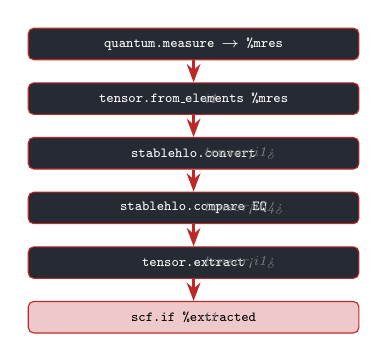
\begin{tikzpicture}[
        node distance=0.28cm,
        box/.style={draw,rounded corners=2pt,minimum width=4.2cm,
                    minimum height=0.40cm,font=\tiny,text centered,
                    fill=codebg,text=white,draw=condred},
        arr/.style={-Stealth,condred,thick},
        lbl/.style={right,font=\tiny,text=gray},
      ]
        \node[box](m1){\texttt{quantum.measure} $\to$ \texttt{\%mres}};
        \node[box,below=of m1](t1){\texttt{tensor.from\_elements \%mres}};
        \node[box,below=of t1](c1){\texttt{stablehlo.convert}};
        \node[box,below=of c1](c2){\texttt{stablehlo.compare EQ}};
        \node[box,below=of c2](t2){\texttt{tensor.extract}};
        \node[box,below=of t2,draw=condred,fill=condred!25,text=black]
          (si){\texttt{scf.if \%extracted}};
        \draw[arr](m1)--(t1)node[lbl]{\textit{i1}};
        \draw[arr](t1)--(c1)node[lbl]{\textit{tensor<i1>}};
        \draw[arr](c1)--(c2)node[lbl]{\textit{tensor<i64>}};
        \draw[arr](c2)--(t2)node[lbl]{\textit{tensor<i1>}};
        \draw[arr](t2)--(si)node[lbl]{\textit{i1}};
      \end{tikzpicture}
      \end{center}
    \column{0.44\textwidth}
      \textbf{How the parser tracks it}

      \smallskip
      The \texttt{ssa\_meas\_source} dictionary propagates the
      measurement index through each forwarding step:

      \vspace{6pt}
      \begin{tabular}{@{}ll@{}}
        \toprule
        Variable & Meas.\ index \\
        \midrule
        \texttt{\%mres} & 1 \\
        \texttt{\%from\_elements} & 1 \\
        \texttt{\%convert} & 1 \\
        \texttt{\%compare} & 1 \\
        \texttt{\%extracted} & 1 \\
        \bottomrule
      \end{tabular}

      \vspace{6pt}
      When \texttt{scf.if \%extracted} is reached, the parser:
      \begin{enumerate}\small
        \item Looks up \texttt{\%extracted} $\Rightarrow$ meas index 1
        \item Parses the then-block for quantum gates
        \item Builds \texttt{ConditionalBlock(meas\_idx=1, then\_gates=[PauliZ])}
      \end{enumerate}
  \end{columns}
\end{frame}

%% ============================================================
\section{Phase 3: QIR Code Generation}
%% ============================================================

\begin{frame}[fragile]{QIR Generator: Ordered Operation Emission}
  \begin{columns}[T]
    \column{0.50\textwidth}
      \begin{lstlisting}[style=pystyle]
def _generate_entry_function(self, circuit, fn):
    body = []
    body.append(
      "  call void"
      " @__quantum__rt__initialize(i8* null)")

    meas_idx = 0
    for op_type, op_data in circuit.ordered_ops:
        if op_type == "gate":
            body.append(
                self._generate_gate_call(op_data))
        elif op_type == "measurement":
            body.append(
                self._generate_measurement(
                    op_data.qubit, meas_idx))
            meas_idx += 1
        elif op_type == "conditional":
            body.extend(
                self._generate_conditional(op_data))

    # Output recording
    body.append(
      f"  call void"
      f" @__quantum__rt__array_record_output"
      f"(i64 {meas_idx}, i8* null)")
      \end{lstlisting}
    \column{0.46\textwidth}
      \textbf{Gate call variants}
      \begin{lstlisting}[style=qirstyle]
; 1-qubit (no parameter)
  call void @__quantum__qis__h__body(
    %Qubit* null)

; 1-qubit (with double parameter)
  call void @__quantum__qis__rx__body(
    double 2.590000e+00,
    %Qubit* inttoptr(i64 1 to %Qubit*))

; 2-qubit gate
  call void @__quantum__qis__cnot__body(
    %Qubit* null,
    %Qubit* inttoptr(i64 1 to %Qubit*))
      \end{lstlisting}

      \vspace{4pt}
      \textbf{Qubit pointer encoding}

      \smallskip
      \begin{tabular}{@{}ll@{}}
        \toprule
        Qubit & QIR pointer \\
        \midrule
        0 & \texttt{\%Qubit* null} \\
        $k > 0$ & \texttt{inttoptr(i64 k to \%Qubit*)} \\
        \bottomrule
      \end{tabular}
  \end{columns}
\end{frame}

\begin{frame}[fragile]{QIR Generator: Conditional Branch Emission}
  \begin{columns}[T]
    \column{0.50\textwidth}
      \begin{lstlisting}[style=pystyle]
def _generate_conditional(self, cond):
    lid = self.conditional_counter
    self.conditional_counter += 1
    suffix = "" if lid == 0 else str(lid)
    result_ptr = get_result_pointer(
        cond.condition_measurement_idx)

    lines = [
      f"  %cond{lid} = call i1"
      f"    @__quantum__qis__read_result__body"
      f"    (%Result* {result_ptr})",
      f"  br i1 %cond{lid},"
      f"    label %then{suffix},"
      f"    label %else{suffix}",
      f"then{suffix}:",
    ]
    for g in cond.then_gates:
        lines.append(self._generate_gate_call(g))
    lines += [
      f"  br label %continue{suffix}",
      f"else{suffix}:",
      f"  br label %continue{suffix}",
      f"continue{suffix}:",
    ]
    return lines
      \end{lstlisting}
    \column{0.46\textwidth}
      \textbf{Generated QIR -- teleportation Z/X corrections}
      \begin{lstlisting}[style=qirstyle]
  %cond0 = call i1
    @__quantum__qis__read_result__body(
      %Result* inttoptr(i64 1 to %Result*))
  br i1 %cond0, label %then, label %else

then:
  call void @__quantum__qis__z__body(
    %Qubit* inttoptr(i64 2 to %Qubit*))
  br label %continue

else:
  br label %continue

continue:
  %cond1 = call i1
    @__quantum__qis__read_result__body(
      %Result* null)
  br i1 %cond1, label %then1, label %else1

then1:
  call void @__quantum__qis__x__body(
    %Qubit* inttoptr(i64 2 to %Qubit*))
  br label %continue1

else1:
  br label %continue1

continue1:
      \end{lstlisting}
  \end{columns}
\end{frame}

\begin{frame}{Gate Mapping: 17 Gates Supported}
  \begin{columns}[T]
    \column{0.50\textwidth}
      \centering\small
      \begin{tabular}{@{}lll@{}}
        \toprule
        Catalyst Gate & QIR function & Type \\
        \midrule
        \texttt{Hadamard}  & \texttt{..h..body}   & 1q \\
        \texttt{PauliX/Y/Z}& \texttt{..x/y/z..}   & 1q \\
        \texttt{S / T}     & \texttt{..s/t..body} & 1q \\
        \texttt{Sdg / Tdg} & \texttt{..sdg/tdg..} & 1q \\
        \texttt{RX}        & \texttt{..rx..body}  & 1q+param \\
        \texttt{RY}        & \texttt{..ry..body}  & 1q+param \\
        \texttt{RZ / PhaseShift} & \texttt{..rz..body} & 1q+param \\
        \texttt{CNOT}      & \texttt{..cnot..}    & 2q \\
        \texttt{CZ}        & \texttt{..cz..body}  & 2q \\
        \texttt{SWAP}      & \texttt{..swap..}    & 2q \\
        \texttt{CY}        & \texttt{..cy..body}  & 2q \\
        \texttt{Toffoli}   & \texttt{..ccx..body} & 3q \\
        \texttt{CSWAP}     & \texttt{..cswap..}   & 3q \\
        \bottomrule
      \end{tabular}
    \column{0.46\textwidth}
      \textbf{Declaration signatures}

      \smallskip
      QIR requires forward declarations for every gate function used.
      The generator collects all gate functions (including those inside
      conditional blocks) and emits correct signatures:

      \vspace{6pt}
      \begin{tabular}{@{}lp{3.8cm}@{}}
        \toprule
        Gate type & Signature \\
        \midrule
        1q, no param & \texttt{void f(\%Qubit*)} \\
        1q+param     & \texttt{void f(double, \%Qubit*)} \\
        2q           & \texttt{void f(\%Qubit*, \%Qubit*)} \\
        Conditional  & \texttt{i1 read\_result(\%Result*)} \\
        \bottomrule
      \end{tabular}

      \vspace{6pt}
      \textbf{Attributes block}
      \begin{itemize}\small
        \item \texttt{"entry\_point"}
        \item \texttt{"required\_num\_qubits"="N"}
        \item \texttt{"required\_num\_results"="M"}
        \item \texttt{qir\_major\_version = 1}
      \end{itemize}
  \end{columns}
\end{frame}

%% ============================================================
\section{Translation Examples}
%% ============================================================

\begin{frame}[fragile]{Example 1: Bell State $|\Phi^+\rangle$ (2 qubits)}
  \begin{columns}[T]
    \column{0.48\textwidth}
      \textbf{Catalyst MLIR input}
      \begin{lstlisting}[style=mlirstyle]
%0 = quantum.alloc( 2)
%1 = quantum.extract %0[ 0]
%out = quantum.custom "Hadamard"() %1

%2 = quantum.extract %0[ 1]
%out_0:2 = quantum.custom "CNOT"()
    %out, %2

%mres, %q = quantum.measure %out_0#0
%mres_1, %q2 = quantum.measure %out_0#1
      \end{lstlisting}
      \textbf{SSA trace}

      \smallskip
      \begin{tabular}{@{}lll@{}}
        \texttt{\%1}      & $\to$ & qubit 0 \\
        \texttt{\%out}    & $\to$ & qubit 0 (post-H)\\
        \texttt{\%2}      & $\to$ & qubit 1\\
        \texttt{\%out\_0\#0} & $\to$ & qubit 0 (control)\\
        \texttt{\%out\_0\#1} & $\to$ & qubit 1 (target)\\
      \end{tabular}
    \column{0.48\textwidth}
      \textbf{Generated QIR}
      \begin{lstlisting}[style=qirstyle]
define void @main() #0 {
entry:
  call void
    @__quantum__rt__initialize(i8* null)
  call void @__quantum__qis__h__body(
    %Qubit* null)
  call void @__quantum__qis__cnot__body(
    %Qubit* null,
    %Qubit* inttoptr(i64 1 to %Qubit*))
  call void @__quantum__qis__mz__body(
    %Qubit* null, %Result* null)
  call void @__quantum__qis__mz__body(
    %Qubit* inttoptr(i64 1 to %Qubit*),
    %Result* inttoptr(i64 1 to %Result*))
  call void
    @__quantum__rt__array_record_output(
      i64 2, i8* null)
  ret void
}
      \end{lstlisting}
  \end{columns}
\end{frame}

\begin{frame}[fragile]{Example 2: 5-Qubit GHZ State}
  \begin{columns}[T]
    \column{0.48\textwidth}
      \textbf{MLIR -- CNOT chain with SSA chaining}
      \begin{lstlisting}[style=mlirstyle]
%out_qubits = quantum.custom
    "Hadamard"() %1
; ssa_qubit["out_qubits"] = 0

%out_qubits_0:2 = quantum.custom
    "CNOT"() %out_qubits, %2
; #0 = 0, #1 = 1

%out_qubits_1:2 = quantum.custom
    "CNOT"() %out_qubits_0#0, %3
; #0 = 0 (traced!), #1 = 2

%out_qubits_2:2 = quantum.custom
    "CNOT"() %out_qubits_1#0, %4
; #0 = 0 (traced!), #1 = 3

%out_qubits_3:2 = quantum.custom
    "CNOT"() %out_qubits_2#0, %5
; #0 = 0 (traced!), #1 = 4
      \end{lstlisting}
    \column{0.48\textwidth}
      \textbf{Generated QIR}
      \begin{lstlisting}[style=qirstyle]
  call void @__quantum__qis__h__body(
    %Qubit* null)
  call void @__quantum__qis__cnot__body(
    %Qubit* null,
    %Qubit* inttoptr(i64 1 to %Qubit*))
  call void @__quantum__qis__cnot__body(
    %Qubit* null,
    %Qubit* inttoptr(i64 2 to %Qubit*))
  call void @__quantum__qis__cnot__body(
    %Qubit* null,
    %Qubit* inttoptr(i64 3 to %Qubit*))
  call void @__quantum__qis__cnot__body(
    %Qubit* null,
    %Qubit* inttoptr(i64 4 to %Qubit*))
      \end{lstlisting}

      \begin{exampleblock}{Key insight}
        All 4 CNOTs correctly emit \texttt{null} (qubit 0) as control,
        traced through the \texttt{\#0} chain:
        \texttt{out\_qubits\_0\#0 $\to$ out\_qubits\_1\#0 $\to$ ...}
      \end{exampleblock}
  \end{columns}
\end{frame}

\begin{frame}[fragile]{Example 3: Quantum Teleportation (3 qubits)}
  \begin{columns}[T]
    \column{0.40\textwidth}
      \textbf{Circuit topology}

      \vspace{6pt}
      \begin{center}
      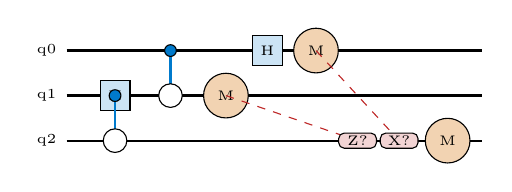
\begin{tikzpicture}[
        wire/.style={draw,-,thick},
        gate/.style={draw,rectangle,minimum size=0.38cm,
                     fill=mlirblue!20,font=\tiny,inner sep=1pt},
        meas/.style={draw,circle,minimum size=0.35cm,
                     fill=ssaorange!30,font=\tiny},
        cond/.style={draw,rectangle,rounded corners=2pt,
                     minimum width=0.48cm,fill=condred!20,
                     font=\tiny,inner sep=1pt},
        scale=0.88
      ]
        \draw[wire](0,0)node[left,font=\tiny]{q0}--+(6,0);
        \draw[wire](0,-0.65)node[left,font=\tiny]{q1}--+(6,0);
        \draw[wire](0,-1.3)node[left,font=\tiny]{q2}--+(6,0);
        \node[gate] at (0.7,-0.65){H};
        \draw[-,thick,mlirblue](0.7,-0.65)--(0.7,-1.3);
        \node[draw,circle,fill=mlirblue,inner sep=1.5pt]
          at (0.7,-0.65){};
        \node[draw,circle,fill=white,inner sep=2pt,
              minimum size=0.3cm] at (0.7,-1.3){};
        \draw[-,thick,mlirblue](1.5,0)--(1.5,-0.65);
        \node[draw,circle,fill=mlirblue,inner sep=1.5pt]
          at (1.5,0){};
        \node[draw,circle,fill=white,inner sep=2pt,
              minimum size=0.3cm] at (1.5,-0.65){};
        \node[meas] at (2.3,-0.65){M};
        \node[gate] at (2.9,0){H};
        \node[meas] at (3.6,0){M};
        \draw[dashed,condred](2.3,-0.65)--(4.2,-1.3);
        \draw[dashed,condred](3.6,0)--(4.8,-1.3);
        \node[cond] at (4.2,-1.3){Z?};
        \node[cond] at (4.8,-1.3){X?};
        \node[meas] at (5.5,-1.3){M};
      \end{tikzpicture}
      \end{center}

      \smallskip
      \small 3 qubits, 3 measurements, 2 conditionals.

      \smallskip
      Z on q2 if M(q1)=1; X on q2 if M(q0)=1
    \column{0.56\textwidth}
      \textbf{Generated QIR (key fragment)}
      \begin{lstlisting}[style=qirstyle]
  call void @__quantum__qis__h__body(
    %Qubit* inttoptr(i64 1 to %Qubit*))
  call void @__quantum__qis__cnot__body(
    %Qubit* inttoptr(i64 1 to %Qubit*),
    %Qubit* inttoptr(i64 2 to %Qubit*))
  call void @__quantum__qis__cnot__body(
    %Qubit* null,
    %Qubit* inttoptr(i64 1 to %Qubit*))
  call void @__quantum__qis__mz__body(
    %Qubit* inttoptr(i64 1 to %Qubit*),
    %Result* null)
  call void @__quantum__qis__h__body(
    %Qubit* null)
  call void @__quantum__qis__mz__body(
    %Qubit* null,
    %Result* inttoptr(i64 1 to %Result*))
  %cond0 = call i1
    @__quantum__qis__read_result__body(
      %Result* inttoptr(i64 1 to %Result*))
  br i1 %cond0, label %then, label %else
then:
  call void @__quantum__qis__z__body(
    %Qubit* inttoptr(i64 2 to %Qubit*))
  br label %continue
      \end{lstlisting}
  \end{columns}
\end{frame}

\begin{frame}[fragile]{Example 4: Parametric Gate -- RX with SSA Constant}
  \begin{columns}[T]
    \column{0.50\textwidth}
      \textbf{Catalyst MLIR}
      \begin{lstlisting}[style=mlirstyle]
%cst = arith.constant 2.590000e+00 : f64
; ssa_constants["cst"] = 2.59

%0 = quantum.alloc( 2)
%1 = quantum.extract %0[ 1]   ; qubit 1
%2 = quantum.extract %0[ 0]   ; qubit 0
%out_q:2 = quantum.custom
    "CNOT"() %1, %2
%out_q0:2 = quantum.custom
    "SWAP"() %out_q#1, %out_q#0
%out_q1 = quantum.custom
    "Hadamard"() %out_q0#1
%out_q2 = quantum.custom
    "S"() %out_q0#0
%out_q3 = quantum.custom
    "RX"(%cst) %out_q2
; params = [2.59] resolved from ssa_constants
%out_q4 = quantum.custom
    "PauliY"() %out_q3
%out_q5:2 = quantum.custom
    "CNOT"() %out_q4, %out_q1
      \end{lstlisting}
    \column{0.46\textwidth}
      \textbf{Generated QIR}
      \begin{lstlisting}[style=qirstyle]
  call void @__quantum__qis__cnot__body(
    %Qubit* inttoptr(i64 1 to %Qubit*),
    %Qubit* null)
  call void @__quantum__qis__swap__body(
    %Qubit* null,
    %Qubit* inttoptr(i64 1 to %Qubit*))
  call void @__quantum__qis__h__body(
    %Qubit* inttoptr(i64 1 to %Qubit*))
  call void @__quantum__qis__s__body(
    %Qubit* null)
  call void @__quantum__qis__rx__body(
    double 2.590000e+00,
    %Qubit* null)
  call void @__quantum__qis__y__body(
    %Qubit* null)
  call void @__quantum__qis__cnot__body(
    %Qubit* null,
    %Qubit* inttoptr(i64 1 to %Qubit*))
      \end{lstlisting}
      \begin{exampleblock}{\small Parameter path}
        \small
        \texttt{\%cst} $\xrightarrow{\text{arith.constant}}$ 2.59
        stored in \texttt{ssa\_constants}.
        Retrieved in \texttt{\_parse\_parameters},
        formatted as \texttt{2.590000e+00} (LLVM notation).
      \end{exampleblock}
  \end{columns}
\end{frame}

%% ============================================================
\section{Phase 4: RAG Knowledge Base}
%% ============================================================

\begin{frame}{RAG System: Retrieval-Augmented Generation}
  \begin{columns}[T]
    \column{0.48\textwidth}
      \textbf{Pipeline}

      \vspace{6pt}
      \begin{center}
      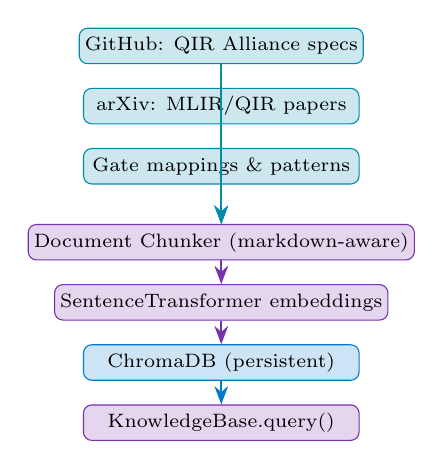
\begin{tikzpicture}[
        node distance=0.3cm,
        box/.style={draw,rounded corners=3pt,minimum width=3.5cm,
                    minimum height=0.45cm,font=\scriptsize,
                    text centered,inner sep=2pt},
        arr/.style={-Stealth,thick},
        src/.style={box,fill=ragcyan!20,draw=ragcyan},
        proc/.style={box,fill=agentpurple!20,draw=agentpurple},
        db/.style={box,fill=mlirblue!20,draw=mlirblue},
      ]
        \node[src](g){GitHub: QIR Alliance specs};
        \node[src,below=of g](a){arXiv: MLIR/QIR papers};
        \node[src,below=of a](e){Gate mappings \& patterns};
        \node[proc,below=0.5cm of e](ch){Document Chunker (markdown-aware)};
        \node[proc,below=of ch](em){SentenceTransformer embeddings};
        \node[db,below=of em](cr){ChromaDB (persistent)};
        \node[proc,below=of cr](kb){KnowledgeBase.query()};
        \draw[arr,ragcyan](g)--(ch);
        \draw[arr,ragcyan](a)--(ch);
        \draw[arr,ragcyan](e)--(ch);
        \draw[arr,agentpurple](ch)--(em);
        \draw[arr,agentpurple](em)--(cr);
        \draw[arr,mlirblue](cr)--(kb);
      \end{tikzpicture}
      \end{center}
    \column{0.48\textwidth}
      \textbf{Knowledge sources}
      \begin{itemize}
        \item \hlc{QIR Alliance GitHub} -- specification docs
        \item \hlc{PennyLane Catalyst} -- dialect documentation
        \item \hlc{CUDA Quantum} -- Quake dialect docs
        \item \hlc{arXiv 2101.11365} -- MLIR for quantum computing
        \item \hlc{arXiv 2303.14500} -- QIR specification paper
        \item Gate mapping reference tables
        \item Translation pattern examples
      \end{itemize}

      \vspace{6pt}
      \textbf{Embedding model}

      \texttt{all-MiniLM-L6-v2} via SentenceTransformers
      (384-dimensional dense vectors)

      \vspace{6pt}
      \textbf{Query interface}

      \texttt{KnowledgeBase.query(text, n=5)}
      returns ranked documents by cosine similarity.
      Used by \texttt{RAGTool} in the agent system.
  \end{columns}
\end{frame}

%% ============================================================
\section{Phase 5: Multi-Agent System}
%% ============================================================

\begin{frame}{Multi-Agent System: CrewAI Orchestration}
  \begin{center}
  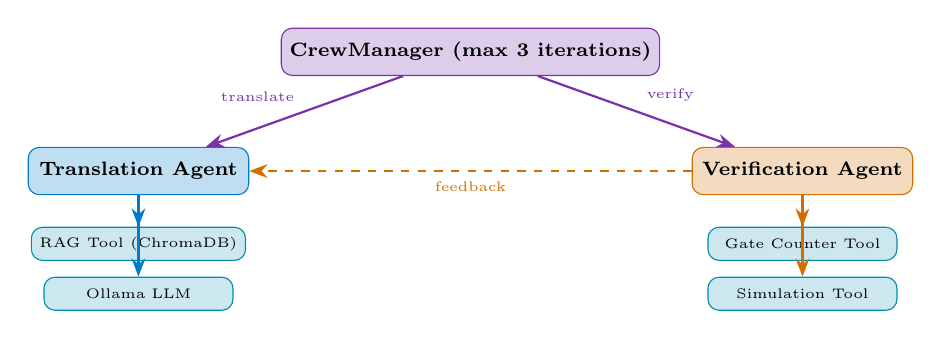
\begin{tikzpicture}[
    node distance=0.45cm and 0.9cm,
    box/.style={draw,rounded corners=4pt,minimum width=2.8cm,
                minimum height=0.6cm,font=\scriptsize\bfseries,
                text centered,inner sep=3pt},
    arr/.style={-Stealth,thick},
    mgr/.style={box,fill=agentpurple!25,draw=agentpurple,
               minimum width=4.2cm},
    ta/.style={box,fill=mlirblue!25,draw=mlirblue},
    va/.style={box,fill=ssaorange!25,draw=ssaorange},
    tool/.style={box,fill=ragcyan!20,draw=ragcyan,
                 minimum width=2.4cm,minimum height=0.42cm,
                 font=\tiny},
  ]
    \node[mgr](crew){CrewManager (max 3 iterations)};
    \node[ta,below left=0.9cm and 0.4cm of crew](ta){Translation Agent};
    \node[va,below right=0.9cm and 0.4cm of crew](va){Verification Agent};
    \node[tool,below=0.4cm of ta](rag){RAG Tool (ChromaDB)};
    \node[tool,below=0.2cm of rag](llm1){Ollama LLM};
    \node[tool,below=0.4cm of va](gc){Gate Counter Tool};
    \node[tool,below=0.2cm of gc](sim){Simulation Tool};
    \draw[arr,agentpurple](crew)--(ta)
      node[midway,above left,font=\tiny]{translate};
    \draw[arr,agentpurple](crew)--(va)
      node[midway,above right,font=\tiny]{verify};
    \draw[arr,ssaorange,dashed](va)--(ta)
      node[midway,below,font=\tiny]{feedback};
    \draw[arr,mlirblue](ta)--(rag);
    \draw[arr,mlirblue](ta)--(llm1);
    \draw[arr,ssaorange](va)--(gc);
    \draw[arr,ssaorange](va)--(sim);
  \end{tikzpicture}
  \end{center}
  \vspace{6pt}
  \begin{columns}[T]
    \column{0.48\textwidth}
      \textbf{TranslationAgent}

      \small Role: MLIR-to-QIR Specialist.
      Uses RAGTool to retrieve relevant specs and patterns,
      then calls Ollama LLM to generate QIR.
      Returns \texttt{TranslationResult} with \texttt{qir\_code},
      \texttt{iterations}, \texttt{success}.
    \column{0.48\textwidth}
      \textbf{VerificationAgent}

      \small Role: QIR Verification Specialist.
      Uses GateCounterTool (exact match) and SimulationTool
      (statistical comparison). Returns feedback dict for
      the next iteration if verification fails.
  \end{columns}
\end{frame}

%% ============================================================
\section{Phase 6: Verification Engine}
%% ============================================================

\begin{frame}{Four-Level Verification Pipeline}
  \begin{center}
  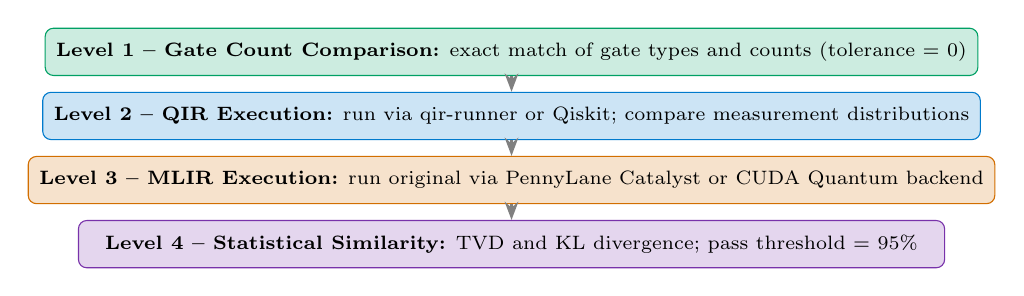
\begin{tikzpicture}[
    level/.style={draw,rounded corners=3pt,minimum width=11cm,
                  minimum height=0.6cm,font=\scriptsize,
                  text centered,inner sep=4pt},
    arr/.style={-Stealth,thick,gray},
  ]
    \node[level,fill=qirgreen!20,draw=qirgreen](l1){%
      \textbf{Level 1 -- Gate Count Comparison:}
      exact match of gate types and counts (tolerance = 0)};
    \node[level,fill=mlirblue!20,draw=mlirblue,
      below=0.2cm of l1](l2){%
      \textbf{Level 2 -- QIR Execution:}
      run via qir-runner or Qiskit; compare measurement distributions};
    \node[level,fill=ssaorange!20,draw=ssaorange,
      below=0.2cm of l2](l3){%
      \textbf{Level 3 -- MLIR Execution:}
      run original via PennyLane Catalyst or CUDA Quantum backend};
    \node[level,fill=agentpurple!20,draw=agentpurple,
      below=0.2cm of l3](l4){%
      \textbf{Level 4 -- Statistical Similarity:}
      TVD and KL divergence; pass threshold = 95\%};
    \draw[arr](l1)--(l2); \draw[arr](l2)--(l3); \draw[arr](l3)--(l4);
  \end{tikzpicture}
  \end{center}
  \vspace{6pt}
  \begin{columns}[T]
    \column{0.50\textwidth}
      \textbf{Simulator registry (plugin-based)}
      \begin{itemize}\small
        \item \texttt{QIRRunner} -- calls \texttt{qir-runner} executable
        \item \texttt{CatalystRunner} -- PennyLane runtime
        \item \texttt{QiskitRunner} -- Qiskit Aer simulator
        \item Add new backends by subclassing \texttt{BaseRunner}
      \end{itemize}
    \column{0.46\textwidth}
      \textbf{Metrics computed}
      \begin{itemize}\small
        \item Total Variation Distance (TVD)
        \item KL divergence (distribution comparison)
        \item Circuit depth estimation
        \item Missing / extra gate reporting
      \end{itemize}
  \end{columns}
\end{frame}

%% ============================================================
\section{Phase 7: Web Interface}
%% ============================================================

\begin{frame}{Streamlit Web Interface}
  \begin{columns}[T]
    \column{0.45\textwidth}
      \textbf{Features}
      \begin{itemize}
        \item 50/50 split layout (MLIR left, QIR right)
        \item 600px monospace text areas
        \item Built-in example loader
        \item LLM model selector (8B / 13B / 70B)
        \item Multi-agent mode toggle
        \item Download generated \texttt{.ll} file
        \item Circuit metrics display
      \end{itemize}

      \vspace{8pt}
      \textbf{Launch}

      \texttt{streamlit run src/ui/app.py}

      \vspace{8pt}
      \textbf{Built-in examples}
      \begin{itemize}\small
        \item Bell State, GHZ-5, Teleportation
        \item Random circuits (658, 6994, \ldots)
      \end{itemize}
    \column{0.51\textwidth}
      \begin{center}
      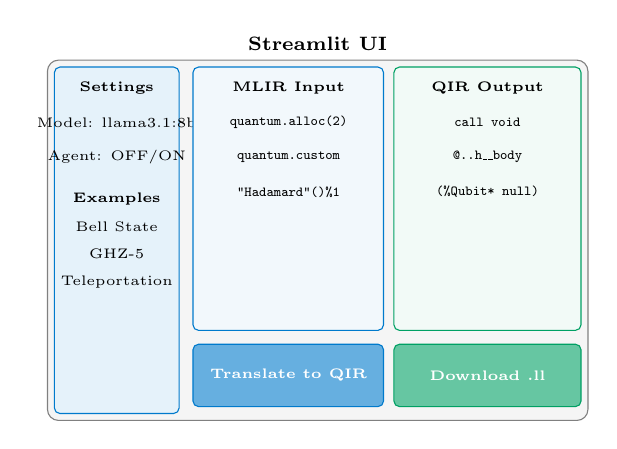
\begin{tikzpicture}[scale=0.88]
        \draw[rounded corners=4pt,draw=gray,fill=gray!8]
          (0,0) rectangle (7.8,5.2);
        \node[above,font=\scriptsize\bfseries] at (3.9,5.2)
          {Streamlit UI};
        %% Sidebar
        \draw[fill=mlirblue!10,draw=mlirblue,rounded corners=2pt]
          (0.1,0.1) rectangle (1.9,5.1);
        \node[font=\tiny\bfseries] at (1.0,4.8){Settings};
        \node[font=\tiny,align=left] at (1.0,4.3)
          {Model: llama3.1:8b};
        \node[font=\tiny,align=left] at (1.0,3.8)
          {Agent: OFF/ON};
        \node[font=\tiny\bfseries] at (1.0,3.2){Examples};
        \node[font=\tiny] at (1.0,2.8){Bell State};
        \node[font=\tiny] at (1.0,2.4){GHZ-5};
        \node[font=\tiny] at (1.0,2.0){Teleportation};
        %% MLIR panel
        \draw[fill=mlirblue!5,draw=mlirblue,rounded corners=2pt]
          (2.1,1.3) rectangle (4.85,5.1);
        \node[font=\tiny\bfseries] at (3.48,4.8){MLIR Input};
        \node[font=\tiny,align=left] at (3.48,4.3)
          {\texttt{quantum.alloc(2)}};
        \node[font=\tiny,align=left] at (3.48,3.8)
          {\texttt{quantum.custom}};
        \node[font=\tiny,align=left] at (3.48,3.3)
          {\texttt{"Hadamard"()\%1}};
        %% QIR panel
        \draw[fill=qirgreen!5,draw=qirgreen,rounded corners=2pt]
          (5.0,1.3) rectangle (7.7,5.1);
        \node[font=\tiny\bfseries] at (6.35,4.8){QIR Output};
        \node[font=\tiny,align=left] at (6.35,4.3)
          {\texttt{call void}};
        \node[font=\tiny,align=left] at (6.35,3.8)
          {\texttt{@..h\_\_body}};
        \node[font=\tiny,align=left] at (6.35,3.3)
          {\texttt{(\%Qubit* null)}};
        %% Buttons
        \draw[fill=mlirblue!60,draw=mlirblue,rounded corners=2pt]
          (2.1,0.2) rectangle (4.85,1.1);
        \node[font=\tiny\color{white}] at (3.48,0.65)
          {\textbf{Translate to QIR}};
        \draw[fill=qirgreen!60,draw=qirgreen,rounded corners=2pt]
          (5.0,0.2) rectangle (7.7,1.1);
        \node[font=\tiny\color{white}] at (6.35,0.65)
          {\textbf{Download .ll}};
      \end{tikzpicture}
      \end{center}
  \end{columns}
\end{frame}

%% ============================================================
\section{Project Structure \& Stack}
%% ============================================================

\begin{frame}[fragile]{Project Structure}
  \begin{columns}[T]
    \column{0.48\textwidth}
      \textbf{Source tree -- 9 packages, 33 modules}
      \begin{lstlisting}[style=pystyle]
src/
  config/       # Settings, LLM model registry
  dialects/     # BaseDialect, Catalyst,
                # Quake, DialectDetector
  parsers/      # MLIRParser
  generators/   # QIRGenerator, QIRTemplates
  agents/       # CrewManager,
                # TranslationAgent,
                # VerificationAgent
  tools/        # RAGTool, GateCounterTool
  rag/          # KnowledgeBase,
                # DocumentFetcher, Chunker
  verification/ # GateCounter, Metrics,
                # SimulatorRegistry, QIRRunner
  ui/           # Streamlit app.py
      \end{lstlisting}
    \column{0.48\textwidth}
      \textbf{Supporting directories}
      \begin{lstlisting}[style=pystyle]
scripts/
  fetch_knowledge.py  # Download docs
  initialize_db.py    # Populate ChromaDB
  setup_llm.sh        # Ollama model pull

knowledge_base/
  qir_specs/  mlir_docs/
  examples/   research/  (arXiv PDFs)

example/mlir/   # Ground-truth MLIR
example/qir/    # Ground-truth QIR (.ll)
data/chromadb/  # Persistent vector DB
docs/diagrams/  # PlantUML (.puml) files
      \end{lstlisting}

      \vspace{4pt}
      \textbf{Quick start}
      \begin{lstlisting}[style=pystyle]
pip install -r requirements.txt
ollama pull llama3.1:8b
python scripts/fetch_knowledge.py
python scripts/initialize_db.py
streamlit run src/ui/app.py
      \end{lstlisting}
  \end{columns}
\end{frame}

\begin{frame}{Technology Stack}
  \begin{center}
  \renewcommand{\arraystretch}{1.25}
  \begin{tabular}{>{\bfseries\color{mlirblue}}p{2.8cm}
                  >{\ttfamily}p{4.2cm}
                  p{5.0cm}}
    \toprule
    Layer & Technology & Role \\
    \midrule
    Language      & Python 3.12
                  & All modules; 33 files; 3\,700+ lines \\
    LLM Backend   & Ollama (local)
                  & Serves models via HTTP API \\
    LLM Models    & llama3.1:8b / 70b-q4
                  & Translation and verification agents \\
    Agent Fw.     & CrewAI
                  & Multi-agent orchestration loop \\
    Vector DB     & ChromaDB (persistent)
                  & RAG document store \\
    Embeddings    & SentenceTransformers
                  & all-MiniLM-L6-v2 (384-dim) \\
    Web UI        & Streamlit
                  & Interactive 50/50 split layout \\
    Configuration & Pydantic + dotenv
                  & Type-safe environment settings \\
    Source IRs    & Catalyst MLIR, Quake MLIR
                  & PennyLane, CUDA Quantum \\
    Target IR     & QIR 1.0 (LLVM IR)
                  & QIR Alliance specification \\
    \bottomrule
  \end{tabular}
  \end{center}
\end{frame}

%% ============================================================
\section{Validation \& Results}
%% ============================================================

\begin{frame}{Validation Results}
  \begin{center}
  \renewcommand{\arraystretch}{1.3}
  \begin{tabular}{@{}lccccl@{}}
    \toprule
    \textbf{Circuit} & \textbf{Qubits} & \textbf{Gates}
      & \textbf{Params} & \textbf{Cond.} & \textbf{Status} \\
    \midrule
    Bell State ($|\Phi^+\rangle$)
      & 2 & H, CNOT & -- & -- & \hlg{\faCheckCircle\ Pass} \\
    5-Qubit GHZ
      & 5 & H, 4$\times$CNOT & -- & -- & \hlg{\faCheckCircle\ Pass} \\
    Quantum Teleportation
      & 3 & 2H, 2CNOT, Z, X & -- & 2 & \hlg{\faCheckCircle\ Pass} \\
    Random Circuit 658
      & 2 & CNOT, SWAP, H, S, RX, Y, CNOT & 2.59 & -- & \hlg{\faCheckCircle\ Pass} \\
    Random Circuit 6994
      & 2 & Various mixed gates & -- & -- & \hlg{\faCheckCircle\ Pass} \\
    \bottomrule
  \end{tabular}
  \end{center}
  \vspace{8pt}
  \begin{columns}[T]
    \column{0.50\textwidth}
      \textbf{Correctness properties verified}
      \begin{itemize}\small
        \item[\hlg{\faCheck}] Gate types and counts match ground truth
        \item[\hlg{\faCheck}] Qubit indices correctly resolved through SSA chains
        \item[\hlg{\faCheck}] Rotation angles preserved in LLVM scientific notation
        \item[\hlg{\faCheck}] Conditionals linked to correct measurement results
        \item[\hlg{\faCheck}] Operation ordering matches source MLIR
      \end{itemize}
    \column{0.46\textwidth}
      \textbf{Previous bugs (all fixed)}
      \begin{itemize}\small
        \item[\hlr{\faTimes}] Trailing-digit heuristic for qubit resolution
        \item[\hlr{\faTimes}] Gates emitted before measurements (wrong order)
        \item[\hlr{\faTimes}] \texttt{scf.if} blocks silently ignored
        \item[\hlr{\faTimes}] \texttt{arith.constant} not tracked for gate parameters
        \item[\hlr{\faTimes}] Missing \texttt{double} in RX/RY/RZ declarations
      \end{itemize}
  \end{columns}
\end{frame}

%% ============================================================
\section{Conclusion}
%% ============================================================

\begin{frame}{Summary}
  \begin{columns}[T]
    \column{0.50\textwidth}
      \textbf{What was built}
      \begin{itemize}
        \item \hl{7-phase} LLM-powered quantum IR translator
        \item \hl{SSA-aware single-pass parser:}
              correctly resolves multi-result ops,
              constant parameters, and measurement-conditional chains
        \item \hl{Ordered operation emission}
              preserves source semantics
        \item \hl{Plugin dialect architecture}
              for extensibility
        \item \hl{RAG knowledge base}
              with ChromaDB and SentenceTransformers
        \item \hl{CrewAI multi-agent loop}
              with 3-iteration refinement
        \item \hl{4-level verification:}
              gate count, QIR exec, MLIR exec, TVD/KL
        \item \hl{Streamlit UI}
              with 50/50 split layout
      \end{itemize}
    \column{0.46\textwidth}
      \begin{alertblock}{Key technical insight}
        MLIR's SSA form hides physical qubit indices behind
        variable chains spanning multiple operations.
        Only a \emph{single-pass dictionary-based tracker} correctly
        resolves qubit indices, constant parameters, and
        measurement-to-conditional linkages.
      \end{alertblock}

      \vspace{6pt}
      \textbf{Supported gates summary}

      \smallskip
      \begin{tabular}{@{}ll@{}}
        1-qubit & H, X, Y, Z, S, T, Sdg, Tdg \\
        1q+param & RX, RY, RZ, PhaseShift \\
        2-qubit & CNOT, CZ, SWAP, CY \\
        3-qubit & Toffoli, CSWAP \\
      \end{tabular}

      \vspace{6pt}
      \textbf{Statistics}

      33 modules~\(\cdot\)~3\,700+ lines~\(\cdot\)~9 packages

      2 dialect adapters~\(\cdot\)~17 supported gates
  \end{columns}
\end{frame}

\begin{frame}[plain]
  \begin{center}
    \vspace{1.8cm}
    {\Large\bfseries\color{mlirblue}
      LLM-Powered Multi-Agent MLIR $\to$ QIR Translator}
    \vspace{0.5cm}

    \rule{9cm}{0.4pt}
    \vspace{0.4cm}

    \badge{mlirblue}{SSA-Aware Parsing}\quad
    \badge{qirgreen}{Ordered Operations}\quad
    \badge{ssaorange}{Parametric Gates}

    \vspace{6pt}
    \badge{condred}{Conditional Branching}\quad
    \badge{agentpurple}{Multi-Agent LLM}\quad
    \badge{ragcyan}{RAG Knowledge}

    \vspace{0.8cm}
    \rule{9cm}{0.4pt}
    \vspace{0.3cm}

    {\small
      33 modules \(\cdot\) 3\,700+ lines \(\cdot\) 9 packages
      \(\cdot\) 17 supported gates}

    \vspace{0.4cm}
    {\small\color{gray}
      Python 3.12 \(\cdot\) CrewAI \(\cdot\) ChromaDB
      \(\cdot\) Ollama \(\cdot\) Streamlit}
  \end{center}
\end{frame}

\end{document}
